\section{Layer-, View-, and Anchor-Dependent Strengths}
\label{sec:point3}
\subsection{Research Question and Contribution}
\label{sec:structured-overview}
ArchAttend modifies intermediate activations of a frozen 3D reconstruction model to increase attention to an architectural anchor~\cite{archworld}. Its intervention strength controls the size of that change. We study whether a single scene-level scalar is too restrictive. Should strength instead depend on the layer's activation and gradient magnitudes (H1), the anchor's visibility in each view (H2), or the anchor category (H3)? The common VGGT intervention is defined in Section~\ref{sec:reference}.

This study constructs and audits a subset of 54 landmarks. It implements three strength rules, reuses shared segmentation masks, and compares reconstruction errors through matched calibration and confirmation experiments. The pretrained model, dataset, supplied anchor choices, and reference attention objective are inherited components. The structured rules do not train the backbone. They use calibration ground truth to select their hyperparameters, but require no reconstruction ground truth when applied to a new landmark.

\subsection{Dataset Construction and Audit}
\label{sec:structured-data}
\subsubsection{Selecting whole landmarks}
ArchWorld contains 396 landmarks. This study uses a frozen partition of 317 development landmarks and 79 landmarks in a separate evaluation pool. We select 54 landmarks from the 317 and do not run the 79-landmark pool in these experiments. The 54-landmark set contains entire landmark identities. The number of photographs used in a reconstruction is determined separately.

We retain a previously frozen set of 40 landmarks and add one example for each of its 13 missing named anchor labels and its missing-label category. Because each landmark has one supplied anchor label, 14 additions are the minimum needed to cover these categories while retaining the original 40. This constraint does not establish 54 as an optimal sample size.

Among the 336 feasible combinations of additions, we choose the set $S$ minimizing
\begin{equation}
 Q(S)=0.35\bar d_S+0.35d_{95,S}
       +0.15\overline{\mathrm{TV}}_S+0.15\overline{\mathrm{KS}}_S.
 \label{eq:structured-subset}
\end{equation}
For each unselected training landmark $x$, $d_S(x)=\min_{s\in S}D(x,s)$ is the distance to its nearest selected landmark. The mean and 95th percentile are evaluated on the 263 unselected training landmarks, excluding selected landmarks' self-distances. The composite distance $D$ equally weights four normalized descriptor families. These comprise full-image VGGT feature means and variation, categorical metadata (building type, region, and anchor), physical extent, and photo-collection properties (image count, duplicates, resolution, and aspect ratio). Normalization uses training landmarks only. The same saved descriptor distances are used for selection and its coverage audit.

The categorical penalty averages total variation over building type, region, and supplied anchor. The numeric penalty averages the Kolmogorov--Smirnov distance over extent, image count, duplicate fraction, and median megapixels. These distances are
\begin{equation}
\mathrm{TV}(p,q)=\tfrac12\sum_k|p_k-q_k|,\qquad
\mathrm{KS}(F,G)=\sup_t|F(t)-G(t)|.
\end{equation}
Equation~\ref{eq:structured-subset} is a constrained coverage-and-balance heuristic. It does not use reconstruction errors or descriptors from the held-out image collections, and it does not enforce proportional category quotas.

\begin{table}[t]
\caption{Distribution gaps for the selected 54 landmarks. Lower is closer. The full-benchmark column is a post-selection metadata audit. Dashes indicate unavailable full-benchmark photo descriptors.}
\label{tab:structured-subset}
\centering
\begin{tabular}{lrr}
\toprule
Attribute / distance & Training (317) & Full (396)\\
\midrule
Building type / TV & 0.0782 & 0.0774\\
Region / TV & 0.0331 & 0.0236\\
Supplied anchor / TV & 0.2017 & 0.1978\\
Extent / KS & 0.0444 & 0.0539\\
Image count / KS & 0.0983 & ---\\
Duplicate fraction / KS & 0.0612 & ---\\
Median megapixels / KS & 0.0721 & ---\\
\bottomrule
\end{tabular}
\end{table}

\subsubsection{What the audit establishes}
The subset covers all nine building types, eight regions, and 25 supplied anchor-label categories in the training partition, including missing labels. Gate and spire occur outside this subset, giving 27 supplied-label categories across the full benchmark. Region proportions are close to the reference populations, while anchor proportions differ more because rare labels were deliberately included (Table~\ref{tab:structured-subset}). For example, windows account for 7.41\% of the subset but 13.56\% of the training landmarks.

The nearest-selected distance on unselected training landmarks has mean 0.50175 and 95th percentile 0.69028 in normalized descriptor units. These quantities measure coverage in the chosen representation. They are not percentages of representativeness or evidence of reconstruction accuracy. They do not certify viewpoint coverage, blur, exposure quality, or unbiased population estimates. Figure~\ref{fig:structured-selection} visualizes the saved distances without replacing them with two-dimensional distances for selection.

\begin{figure*}[t]
\centering
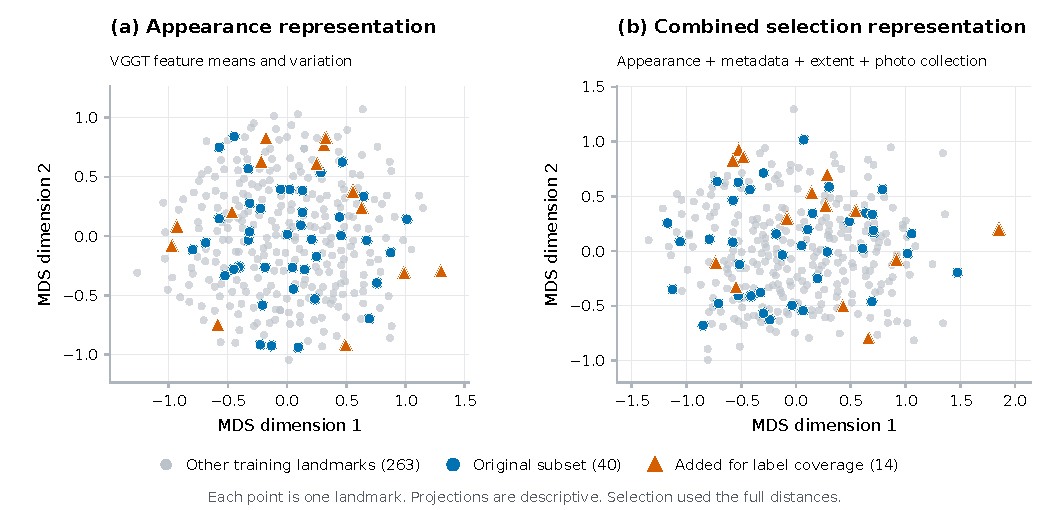
\includegraphics[width=\textwidth]{figures/selection_representations.pdf}
\caption{Selection diagnostics inherited from the completed subset audit. Metric multidimensional scaling projects the appearance distance (left) and the composite distance (right). The original 40 and 14 additions are distinguished from the other 263 training landmarks. Selection used the original distances. Proximity in these two-dimensional projections is approximate. These are data-selection visualizations, not reconstruction results.}
\Description{Two maps of 317 training landmarks distinguish the original forty, fourteen additions, and unselected landmarks, under appearance and composite distances.}
\label{fig:structured-selection}
\end{figure*}

\subsubsection{Calibration, confirmation, and image sampling}
A metadata-only search over 512 candidate allocations, using seed 1729, freezes 18 calibration and 36 internal confirmation landmarks. It favors anchor and region coverage and distribution balance. Supported anchor types retain at least two calibration examples and one confirmation example. Hyperparameters minimize mean calibration error and are frozen before confirmation. The confirmation landmarks are the reporting cohort, not additional tuning examples.

The selection audit records 14,333 source photographs across the 54 landmarks. Reconstruction uses seeded uniform sampling of up to 50 distinct registered images with matching depth and validity data per landmark. All eligible images are retained when fewer than 50 are available, with a minimum of two. Landmarks are neither padded nor replaced. The actual experiments use 2,622 images in total, including 1,776 confirmation images. Counts range from 19 to 50 across the full subset. The confirmation set includes the 26-view Bell Tower of Vank Cathedral and 35 landmarks with 50 views. Images are repeated measurements within a landmark, not independent evaluation samples.

SAM 3 masks are prepared once and reused by all hypotheses. Supplied anchors are retained except for documented manual corrections, namely bridge for Forth Bridge and obelisk for Washington Monument, whose supplied altar label produced empty masks. The corrections retain the landmark split. The selection audit uses the original supplied labels. Numeric mask validation is complete, but semantic review of all saved overlays remains necessary before architectural claims.

\subsection{Structured Intervention Rules}
\label{sec:structured-rules}
All hypotheses preserve the objective, layer range, one-step update, and accept/revert rule. They change the coefficient multiplying the gradient. Anchor masks define the objective and, for H1, the norms. The resulting gradient update is applied across all tokens rather than being restricted to anchor tokens. Empty anchor masks produce no update.

\subsubsection{H1 layer-dependent relative strength}
Layer activation and gradient magnitudes can differ, so a fixed coefficient need not yield a comparable relative perturbation at each layer. We set
\begin{equation}
 \eta_l=\min\!\left(10^5,
 \frac{\alpha\|T_l[M]\|_2}{\max(\|g_l[M]\|_2,10^{-8})}\right),
 \qquad \alpha\in\{0.01,0.02\}.
 \label{eq:structured-h1}
\end{equation}
Empty masks and zero masked gradients give a zero step. Before clipping and acceptance, this targets an anchor-masked update magnitude of approximately $\alpha$ times the masked activation magnitude. Here $\alpha$ is a relative-strength hyperparameter. It is not directly comparable numerically to scalar $\eta$.

\subsubsection{H2 view-dependent strength}
Let $n_v$ be the number of anchor tokens in view $v$ at the first intervention hook, and let $\bar n$ be their mean across views. Define
\begin{equation}
 q_v=\operatorname{clip}\!\left(\sqrt{\frac{n_v+1}{\bar n+1}},0.5,2\right),
 \qquad \eta_v=\frac{\eta q_v}{\sqrt{V^{-1}\sum_{u=1}^{V}q_u^2}},
 \label{eq:structured-h2}
\end{equation}
with base $\eta\in\{100,1000\}$. Views with more anchor tokens receive larger coefficients. The weights are fixed across layers so that this tests view-dependent rather than jointly layer-and-view-dependent coefficients. RMS normalization gives $V^{-1}\sum_v\eta_v^2=\eta^2$ when an anchor is present. It preserves the RMS coefficient, not the norm of the resulting gradient update or its reconstruction effect.

\subsubsection{H3 anchor-dependent strength}
For an anchor category $a$ with calibration set $\mathcal C_a$, choose
\begin{equation}
 \eta_a^*=\arg\min_{\eta\in\{100,1000\}}
      \frac{1}{|\mathcal C_a|}\sum_{s\in\mathcal C_a}C_s(\eta),
 \qquad |\mathcal C_a|\ge2,
 \label{eq:structured-h3}
\end{equation}
where $C_s$ is normalized Chamfer error. For categories with fewer than two calibration landmarks, use the globally selected scalar from the same grid. H3 is a frozen lookup at inference time. It does not select $\eta$ using the new landmark's ground-truth reconstruction.

The six types with enough calibration support are arch, column, facade, statue, tower, and window. Column and statue select $\eta=100$. The other supported types select $\eta=1000$. Every fallback type also uses $\eta=1000$. Table~\ref{tab:structured-anchor-selection} reports the calibration means and sample counts. Dome and minaret are fallback types. This study does not estimate separate successful rules for those categories.

\begin{table*}[t]
\caption{H3 calibration and frozen choices. Each error is a mean over calibration landmarks of that anchor type. Confirmation counts describe where the frozen choices are evaluated. They do not enter selection. The remaining 19 confirmation landmarks use the global-scalar fallback.}
\label{tab:structured-anchor-selection}
\centering
\begin{tabular}{lrrrrr}
\toprule
Anchor & Calibration $n$ & Confirmation $n$ & Mean at $\eta=100$ & Mean at $\eta=1000$ & Selected $\eta$ \\
\midrule
Arch & 6 & 8 & 14.86956 & 11.95316 & 1000 \\
Column & 3 & 1 & 7.43322 & 9.75595 & 100 \\
Facade & 2 & 3 & 15.62376 & 10.79510 & 1000 \\
Statue & 2 & 2 & 9.36013 & 9.67054 & 100 \\
Tower & 2 & 1 & 7.82095 & 7.68955 & 1000 \\
Window & 2 & 2 & 5.95998 & 5.55834 & 1000 \\
\bottomrule
\end{tabular}

\end{table*}

\subsection{Experimental Protocol}
\label{sec:structured-evaluation}
We use the metric defined in Section~\ref{sec:task} and evaluate all hypotheses on the same 36 confirmation landmarks.

All three studies select the same global scalar, $\eta=1000$. Its mean calibration error is 9.68941, compared with 10.84976 for $\eta=100$. H1 selects $\alpha=0.02$ (10.26246 versus 11.52723 for $\alpha=0.01$). H2 selects base $\eta=100$ (9.96551 versus 10.69762 for base $\eta=1000$). These choices optimize each method's own candidate set. The independently selected H2 base and scalar control differ, so their comparison does not isolate view weighting at equal base strength.

The experiments use NVIDIA L4 GPUs, float32 model weights with the reference autocast behavior, and seed 1729. The runner verifies fresh-reference equivalence, input identities, checkpoint integrity, view counts, metric normalization, and frozen calibration choices before accepting results. Resume checks require the recorded source and hardware/software profile. The final combined validation passed on November 24, 2026. All three studies use the same confirmation cohort, ordered images, masks, hardware/software, and shared control predictions and metrics.

Each hypothesis completes all 54 landmarks with no unresolved failures. H1 and H2 each contain 198 completed scene/condition jobs. H3 contains 129, for 525 across the independent studies, excluding extra reference checks. Controls are repeated across studies. H3 reuses identical condition outputs when its lookup selects the global scalar. Its number of distinct jobs therefore falls below the three-condition-per-confirmation-landmark upper bound. These counts establish completion, not a wall-time speedup or equal computational cost across methods.

\subsection{Results}
\label{sec:structured-results}
\subsubsection{Overall comparison}
Table~\ref{tab:structured-main} gives the absolute errors, and Table~\ref{tab:structured-paired} gives paired effects. H1 has the lowest mean among the intervention methods, while no intervention has the lowest mean overall. H1 also has the lowest median. A lower median alongside a higher mean indicates that typical-scene improvements can coexist with large degradations on a smaller number of landmarks.

\begin{table}[t]
\caption{Confirmation error on 36 landmarks. Lower is better. The no-intervention baseline has the best mean. H1 has the best median.}
\label{tab:structured-main}
\centering
\begin{tabular}{lrr}
\toprule
Condition & Mean normalized CD & Median \\
\midrule
No intervention & 13.92426 & 7.35234 \\
Global scalar ($\eta=1000$) & 14.76303 & 6.84867 \\
H1 per-layer ($\alpha=0.02$) & 14.14062 & 6.57717 \\
H2 per-view (base $\eta=100$) & 14.76697 & 6.99407 \\
H3 per-anchor & 14.40769 & 6.84867 \\
\bottomrule
\end{tabular}

\end{table}

\begin{table*}[p]
\caption{Paired confirmation differences. W/T/L denotes improved/tied/worsened landmarks relative to the scalar. Negative differences favor the structured method. Percentage changes reported in the text are ratios of cohort means, not averages of per-landmark percentages.}
\label{tab:structured-paired}
\centering
\begin{tabular}{lrrrr}
\toprule
Method & Mean vs. scalar & Median vs. scalar & W/T/L vs. scalar & Mean vs. no intervention \\
\midrule
H1 & -0.62241 & -0.04327 & 23/0/13 & +0.21637 \\
H2 & +0.00394 & +0.05177 & 13/0/23 & +0.84272 \\
H3 & -0.35533 & +0.00000 & 2/33/1 & +0.48344 \\
\bottomrule
\end{tabular}

\end{table*}

\begin{figure*}[p]
\centering
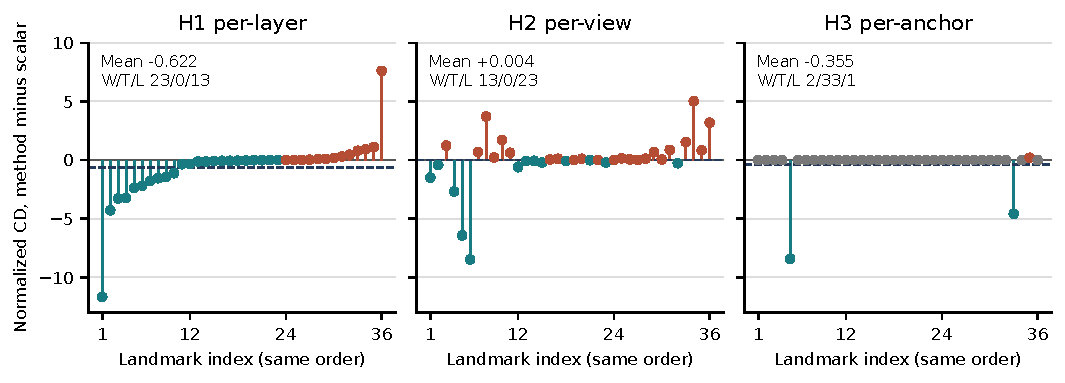
\includegraphics[width=\textwidth]{figures/paired_effects.pdf}
\caption{Per-landmark differences from the global scalar. All panels use the same landmark order, sorted by H1's difference, and the same vertical scale. Teal points improve, orange points worsen, gray points tie, and dashed lines show means. H3 changes only three predictions, whereas H1 and H2 change all 36.}
\Description{Three panels plot paired effects across thirty-six landmarks. H1 has twenty-three improvements and thirteen regressions. H2 has thirteen improvements and twenty-three regressions. H3 has two improvements, thirty-three ties, and one regression.}
\label{fig:structured-paired}
\end{figure*}

\subsubsection{Exploratory analysis by anchor label}
The 36 confirmation landmarks contain 23 distinct executed anchor labels. The six groups containing multiple landmarks are arch ($n=8$), facade ($n=3$), and bridge, pillar, statue, and window ($n=2$ each). These account for 19 landmarks. Each of the other 17 labels occurs once. We use the recorded intervention labels, including the documented corrections, and retain distinctions such as pillar versus column and tower versus bell tower. These are label-based groups, not an independent verification of the architectural elements in each image.

For anchor group $a$, method $h$, and reference $r$, we report
\begin{equation}
 R_{a,h\mid r}=100\left(\frac{\bar C_{a,h}}{\bar C_{a,r}}-1\right),
 \qquad
 \bar C_{a,h}=\frac{1}{n_a}\sum_{s\in a}C_{s,h}.
\end{equation}
Negative values indicate lower group mean error. Each landmark has equal weight within its group. Percentages are ratios of group means. They are not averages of per-landmark percentages. Table~\ref{tab:structured-all-anchors} includes every group for all three hypotheses, and Table~\ref{tab:structured-anchor-wins} records wins, ties, and losses in the six groups with multiple landmarks. Figure~\ref{fig:structured-anchor-groups} visualizes their mean changes against both references.

The outcome is whole-landmark reconstruction error, not error restricted to the segmented anchor. An improvement for facade-labeled landmarks therefore does not by itself establish better reconstruction of facade pixels or points. This is a post-hoc descriptive analysis of frozen confirmation outputs. It neither changes the calibrated policies nor fits a new method selector using the confirmation results.

\begin{table*}[p]
\caption{All 23 confirmation anchor labels. Entries are percentage changes in group mean normalized Chamfer error versus the scalar or no intervention. Negative is better. The divider separates repeated groups from individual cases. H3's zero scalar-relative changes are exact prediction ties.}
\label{tab:structured-all-anchors}
\centering
\begin{tabular}{lr rrrrrr}
\toprule
& & \multicolumn{2}{c}{H1} & \multicolumn{2}{c}{H2} & \multicolumn{2}{c}{H3} \\
\cmidrule(lr){3-4}\cmidrule(lr){5-6}\cmidrule(lr){7-8}
Anchor & $n$ & Scalar & No inter. & Scalar & No inter. & Scalar & No inter. \\
\midrule
Arch & 8 & +0.63 & +1.90 & +7.37 & +8.73 & 0.00 & +1.26 \\
Facade & 3 & -12.83 & -16.80 & +3.60 & -1.11 & 0.00 & -4.55 \\
Bridge & 2 & +1.54 & +2.86 & +6.05 & +7.43 & 0.00 & +1.30 \\
Pillar & 2 & +1.63 & +1.14 & -1.66 & -2.14 & 0.00 & -0.48 \\
Statue & 2 & -3.03 & +1.76 & -13.49 & -9.22 & -19.86 & -15.90 \\
Window & 2 & -0.20 & -3.01 & +1.05 & -1.80 & 0.00 & -2.82 \\
\midrule
Belfry & 1 & -1.20 & +1.14 & -0.58 & +1.77 & 0.00 & +2.37 \\
Bell tower & 1 & +2.26 & -1.47 & +14.17 & +10.01 & 0.00 & -3.64 \\
Column & 1 & +3.70 & +30.63 & +7.14 & +34.98 & -21.27 & -0.82 \\
Dome & 1 & -2.94 & +39.11 & +7.06 & +53.44 & 0.00 & +43.32 \\
Door & 1 & -0.48 & -2.13 & +0.47 & -1.19 & 0.00 & -1.66 \\
Minaret & 1 & -19.33 & -11.99 & -2.47 & +6.39 & 0.00 & +9.09 \\
Obelisk & 1 & -5.70 & -15.84 & +8.68 & -3.01 & 0.00 & -10.76 \\
Pagoda & 1 & +44.72 & +36.25 & +18.77 & +11.82 & 0.00 & -5.85 \\
Pediment & 1 & -0.88 & -1.27 & -1.27 & -1.65 & 0.00 & -0.39 \\
Pyramid & 1 & -6.77 & -8.97 & +2.56 & +0.14 & 0.00 & -2.36 \\
Railing & 1 & -9.25 & +20.50 & -35.89 & -14.87 & 0.00 & +32.78 \\
Relief & 1 & -10.91 & -6.07 & -1.05 & +4.32 & 0.00 & +5.43 \\
Roof & 1 & -2.51 & +0.11 & -3.70 & -1.12 & 0.00 & +2.68 \\
Solomonic column & 1 & +3.40 & -5.76 & +4.18 & -5.05 & 0.00 & -8.86 \\
Stone & 1 & -0.87 & +2.39 & -2.95 & +0.24 & 0.00 & +3.29 \\
Tower & 1 & -13.40 & -13.49 & -11.11 & -11.20 & 0.00 & -0.10 \\
Walkway & 1 & -3.30 & -1.36 & -2.20 & -0.24 & 0.00 & +2.01 \\
\bottomrule
\end{tabular}

\end{table*}

\begin{table*}[p]
\caption{Improved/tied/worsened landmark counts in the six groups with multiple landmarks, versus each reference. H1 improves all facades against both controls. H3 improves both statues against no intervention but only one against the scalar.}
\label{tab:structured-anchor-wins}
\centering
\begin{tabular}{lr cccccc}
\toprule
& & \multicolumn{2}{c}{H1} & \multicolumn{2}{c}{H2} & \multicolumn{2}{c}{H3} \\
\cmidrule(lr){3-4}\cmidrule(lr){5-6}\cmidrule(lr){7-8}
Anchor & $n$ & Scalar & No inter. & Scalar & No inter. & Scalar & No inter. \\
\midrule
Arch & 8 & 3/0/5 & 3/0/5 & 1/0/7 & 2/0/6 & 0/8/0 & 4/0/4 \\
Facade & 3 & 3/0/0 & 3/0/0 & 0/0/3 & 3/0/0 & 0/3/0 & 3/0/0 \\
Bridge & 2 & 1/0/1 & 1/0/1 & 0/0/2 & 1/0/1 & 0/2/0 & 1/0/1 \\
Pillar & 2 & 1/0/1 & 1/0/1 & 2/0/0 & 2/0/0 & 0/2/0 & 1/0/1 \\
Statue & 2 & 1/0/1 & 1/0/1 & 1/0/1 & 2/0/0 & 1/0/1 & 2/0/0 \\
Window & 2 & 1/0/1 & 2/0/0 & 0/0/2 & 2/0/0 & 0/2/0 & 2/0/0 \\
\bottomrule
\end{tabular}

\end{table*}

\begin{figure*}[p]
\centering
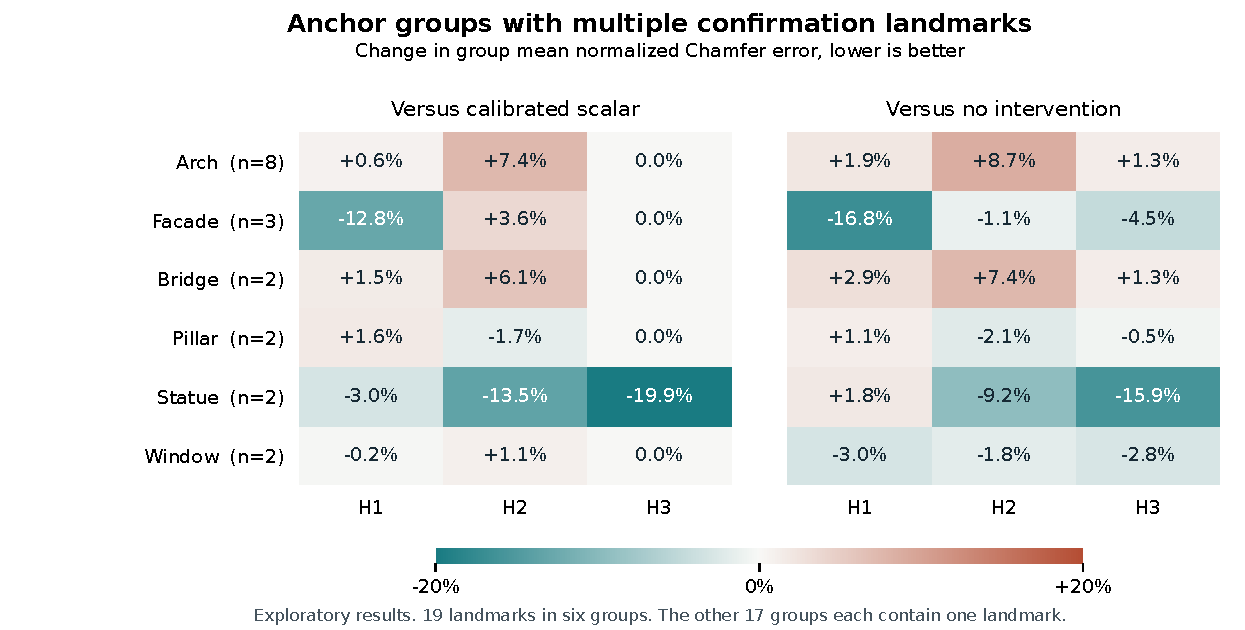
\includegraphics[width=\textwidth]{anchor_analysis/repeated_anchor_groups.pdf}
\caption{Exploratory anchor-group effects for all three hypotheses. Teal indicates lower mean error and orange higher mean error. The panels distinguish improvement over the calibrated intervention from improvement over no intervention. Sample sizes are shown explicitly. None exceeds eight.}
\Description{Two heatmaps show percentage changes for H1, H2, and H3 in the arch, facade, bridge, pillar, statue, and window groups, versus scalar and versus no intervention.}
\label{fig:structured-anchor-groups}
\end{figure*}

\subsubsection{H1 the broadest benefit over the scalar}
H1's mean error is 14.14062, compared with 14.76303 for the global scalar. The mean paired difference is $-0.62241$, a 4.22\% reduction in the cohort mean, with 23 wins and 13 losses. Its median paired difference is $-0.04327$, and its median absolute error is 6.57717. The effect is therefore not a uniform improvement. The individual scalar-relative differences range from $-11.66459$ to $+7.60658$.

Relative to no intervention, H1 improves 21 landmarks and worsens 15, but its mean is 0.21637 higher (1.55\%). Thus the tested layer normalization improves the scalar intervention in this cohort without establishing a lower mean error than the unmodified model.

\paragraph{Anchor groups.}
Facades show the clearest consistent improvement. Their mean error falls from 8.52529 under the scalar to 7.43122, a 12.83\% reduction, and is 16.80\% below no intervention. Herald Square, Jahangiri Mahal, and Patan Durbar Square all improve against both controls. Windows have a smaller mean improvement of 0.20\% over the scalar and 3.01\% over no intervention. One of two improves against the scalar, while both improve against no intervention. Statues improve by 3.03\% in mean relative to the scalar but remain 1.76\% worse than no intervention, with one win and one loss against each control.

The other repeated groups do not improve in mean. For arches, H1 raises mean error by 0.63\% over the scalar and 1.90\% over no intervention, with three wins and five losses against each. Bridge means rise by 1.54\% and 2.86\%, respectively, and pillar means by 1.63\% and 1.14\%. Both groups split into one improvement and one regression. Thus the aggregate H1 benefit does not hold uniformly across anchor labels.

\paragraph{Individual cases and large errors.}
The largest scalar-relative reduction occurs at Place Jacques-Cartier, whose recorded anchor label is minaret. Error falls from 60.35861 to 48.69402 ($\Delta=-11.66459$). It also improves over no intervention, 55.33049. The largest scalar-relative regression occurs at Heian-jing\={u}, labeled pagoda. Error rises from 17.00835 to 24.61493 ($\Delta=+7.60658$), also above its no-intervention value of 18.06564. The largest degradation against no intervention occurs at Pal\'acio Nereu Ramos, labeled dome. 36.77017 rises to 51.15252. These single-landmark groups illustrate both gains and failure cases. They do not establish category-wide effects. Their label semantics also remain subject to mask review.

\subsubsection{H2 no improvement over the scalar mean}
H2's mean error is 14.76697. Its mean paired difference from the scalar is $+0.00394$, or +0.03\% after rounding, while its median paired difference is $+0.05177$. It improves 13 landmarks and worsens 23. The nearly equal means obscure opposing scene-specific changes. They do not imply equivalent predictions. The comparison provides no mean-error benefit for the tested view-dependent rule. Its mean also exceeds no intervention by 0.84272 (6.05\%). Because the calibrated base strengths differ, this result applies to the two selected policies rather than proving that all view weighting is ineffective.

\paragraph{Anchor groups.}
Pillars are the only repeated group in which H2 improves every landmark against both references. Hassan Tower and Taipei Confucius Temple both improve, giving mean reductions of 1.66\% versus the scalar and 2.14\% versus no intervention. Statues show larger mean reductions of 13.49\% and 9.22\%, respectively. Both statues improve over no intervention, but only Marine Corps War Memorial improves over the scalar. Mansudae Grand Monument worsens. The statue mean therefore combines a large gain with a smaller regression against the scalar.

Facades and windows expose the importance of the comparator. H2 improves all three facades and both windows relative to no intervention, with group mean reductions of 1.11\% and 1.80\%. However, every one of those five landmarks is worse under H2 than under the scalar, increasing the two group means by 3.60\% and 1.05\%. Arches and bridges worsen in mean against both controls. Seven of eight arches and both bridges worsen against the scalar. Their mean increases are 7.37\% and 6.05\%. Relative to no intervention, the increases are 8.73\% and 7.43\%.

\paragraph{Offsetting effects.}
The largest scalar-relative gain is at Itmad-Ud-Daulah's Tomb, labeled railing. 23.62690 falls to 15.14755 ($\Delta=-8.47935$), below its no-intervention error of 17.79411. The largest scalar-relative loss is at Saint Demetrius Church in Vladimir, labeled arch. 22.71553 rises to 27.74651 ($\Delta=+5.03098$). Across all 36 landmarks, the sum of error reductions against the scalar is 20.97546, almost canceled by 21.11744 of increases. Against no intervention, H2 wins on 20 landmarks and loses on 16, but the largest loss, at the dome-labeled Pal\'acio Nereu Ramos, is 19.64978. Its error rises from 36.77017 to 56.41995. A majority of small wins therefore coexists with a worse mean.

\subsubsection{H3 a narrow, concentrated improvement}
H3's mean error is 14.40769, reducing the scalar mean by 0.35533 (2.41\%). Its median absolute error remains 6.84867, and its median paired difference is exactly zero. There are two wins, 33 ties, and one loss against the scalar. The 33 ties are explained by the frozen policy. These landmarks use the same scalar condition and prediction, rather than merely obtaining similar scores.

Of the 36 confirmation landmarks, 17 have supported anchor categories and 19 use the fallback. Only two statues and one column receive a coefficient different from the global scalar. Figure~\ref{fig:structured-h3} shows their scores. For Marine Corps War Memorial, $\eta=100$ lowers error from 36.43411 to 28.02065 ($\Delta=-8.41346$). For Palacio Legislativo, Uruguay, it lowers error from 21.53219 to 16.95222 ($\Delta=-4.57996$). For Mansudae Grand Monument, it raises error from 4.91413 to 5.11550 ($\Delta=+0.20137$). These three differences account for the entire cohort-level benefit.

\begin{figure*}[p]
\centering
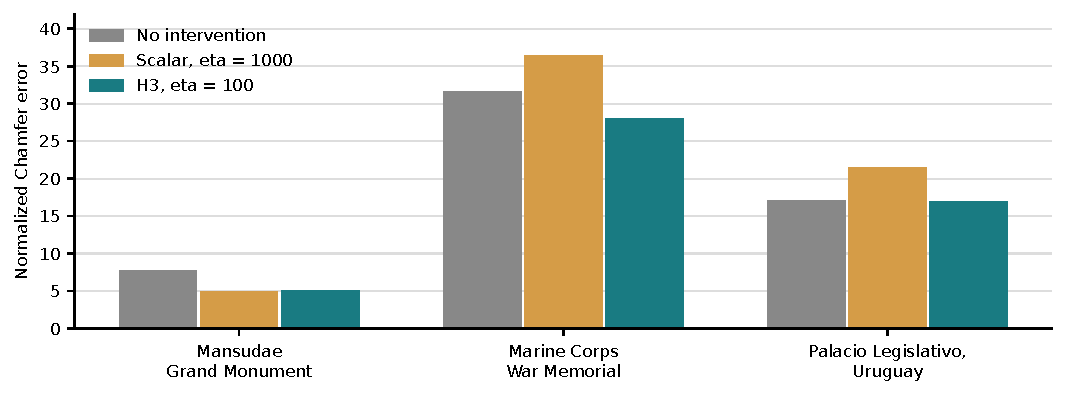
\includegraphics[width=\textwidth]{figures/h3_changed_landmarks.pdf}
\caption{The three confirmation landmarks where H3 selects $\eta=100$ instead of the scalar's $\eta=1000$. Both methods use the same images and masks. Two large improvements and one small regression determine H3's mean difference. The other 33 landmarks are exact scalar ties.}
\Description{Grouped bars compare no intervention, scalar one thousand, and anchor-selected one hundred on Mansudae Grand Monument, Marine Corps War Memorial, and Palacio Legislativo in Uruguay.}
\label{fig:structured-h3}
\end{figure*}

Across supported-anchor confirmation landmarks the mean difference is $-0.75247$, but this still reflects only those three changed predictions. It is not evidence of a broad improvement across all supported categories. H3 remains 0.48344 worse than no intervention in mean error (3.47\%).

\paragraph{Anchor groups and inherited scalar behavior.}
For statues, H3 lowers the group mean from 20.67412 under the scalar to 16.56808, a 19.86\% reduction. This is also 15.90\% below no intervention, whose mean is 19.70144. Both statue landmarks improve over no intervention, while the scalar comparison contains one win and one loss. The only column landmark, Palacio Legislativo, improves by 21.27\% over the scalar but just 0.82\% over no intervention. The difference between those percentages shows that much of the gain corrects the large scalar step's degradation in this case.

For every other anchor label, H3 exactly reuses the scalar prediction. Its improvements over no intervention on facades (4.55\%), windows (2.82\%), and pillars (0.48\%) are therefore inherited scalar effects, not additional gains from choosing strength by category. Likewise, it retains the scalar's mean degradations on arches (1.26\%) and bridges (1.30\%), and its large dome-labeled error at Pal\'acio Nereu Ramos. Overall H3 improves 22 landmarks and worsens 14 against no intervention. The results support a limited effect from the two category choices that differ from the scalar, rather than a broad improvement across the 23 labels.

\subsubsection{Sensitivity and interpretation across hypotheses}
To assess dependence on individual cases, we recompute each cohort mean paired difference after omitting each landmark in turn, without refitting any policy. Table~\ref{tab:structured-sensitivity} gives the minimum and maximum across the 36 resulting sets of 35 landmarks. These are descriptive sensitivity ranges, not confidence intervals or revised headline results.

H1's mean advantage over the scalar remains negative after any single omission, ranging from $-0.85752$ to $-0.30692$. H3 also retains a negative scalar-relative mean, ranging from $-0.37124$ to $-0.12510$, despite its effect being concentrated in three cases. H2's range crosses zero, consistent with its nearly canceled gains and losses. Against no intervention, H1's range crosses zero, while H2 and H3 remain worse in mean after every single omission. The complete 36-landmark means remain the primary results for all methods.

The repeated-group findings motivate further evaluation of H1 on facade-labeled landmarks and H2 on pillar-labeled landmarks. H3 offers a larger but mixed statue-group effect and one column case. These observations were identified after viewing confirmation errors. They are not a validated anchor-to-method selection rule. Testing such a rule would require a separate calibration procedure and new confirmation landmarks or a properly nested evaluation. Retrospective selection audits are reported separately in Section~\ref{sec:complete-selection}. They are not part of the original frozen study.

\begin{table*}[p]
\caption{Mean paired error ranges after omitting each confirmation landmark in turn, with 35 landmarks per calculation and the policy fixed. Negative favors the method. These are sensitivity ranges, not confidence intervals.}
\label{tab:structured-sensitivity}
\centering
\begin{tabular}{lrr}
\toprule
Method & Vs. scalar & Vs. no intervention \\
\midrule
H1 & $[-0.85752, -0.30692]$ & $[-0.18838, +0.41216]$ \\
H2 & $[-0.13969, +0.24632]$ & $[+0.30537, +0.94381]$ \\
H3 & $[-0.37124, -0.12510]$ & $[+0.04210, +0.59985]$ \\
\bottomrule
\end{tabular}

\end{table*}

% Anastasios Gerasis: completed analysis of the frozen confirmation results.
\subsection{Uncertainty and Exploratory Associations}
\label{sec:extended-analysis}
\paragraph{Paired uncertainty.}
We resample the 36 confirmation landmarks as paired units, retaining each landmark's method and reference scores together. With 100,000 bootstrap replicates and seed 20261126, all six pointwise 95\% percentile intervals for mean differences include zero (Table~\ref{tab:bootstrap}). None of six exact two-sided win/loss sign tests survives Holm correction. Tied pairs are excluded from those tests. These findings do not establish equivalence. Resampling this deliberately selected cohort describes uncertainty conditional on its composition and does not certify coverage for the 396-landmark population.

\begin{table*}[t]
\caption{Paired mean differences and bootstrap uncertainty on 36 confirmation landmarks. Negative favors the structured rule. W/T/L denotes improved/tied/worsened landmarks. Intervals are pointwise, not simultaneous. Every interval includes zero.}
\label{tab:bootstrap}
\centering
\begin{tabular}{llrrr}
\toprule
Rule & Reference & Mean $\Delta$ & Pointwise 95\% interval & W/T/L\\
\midrule
H1 & Original & $+0.2164$ & $[-0.7849, +1.4040]$ & 21/0/15\\
H1 & Scalar & $-0.6224$ & $[-1.5247, +0.1813]$ & 23/0/13\\
H2 & Original & $+0.8427$ & $[-0.1018, +2.2123]$ & 20/0/16\\
H2 & Scalar & $+0.0039$ & $[-0.7783, +0.6863]$ & 13/0/23\\
H3 & Original & $+0.4834$ & $[-0.3451, +1.6351]$ & 22/0/14\\
H3 & Scalar & $-0.3553$ & $[-0.9500, +0.0112]$ & 2/33/1\\
\bottomrule
\end{tabular}

\end{table*}

\begin{figure*}[t]
\centering
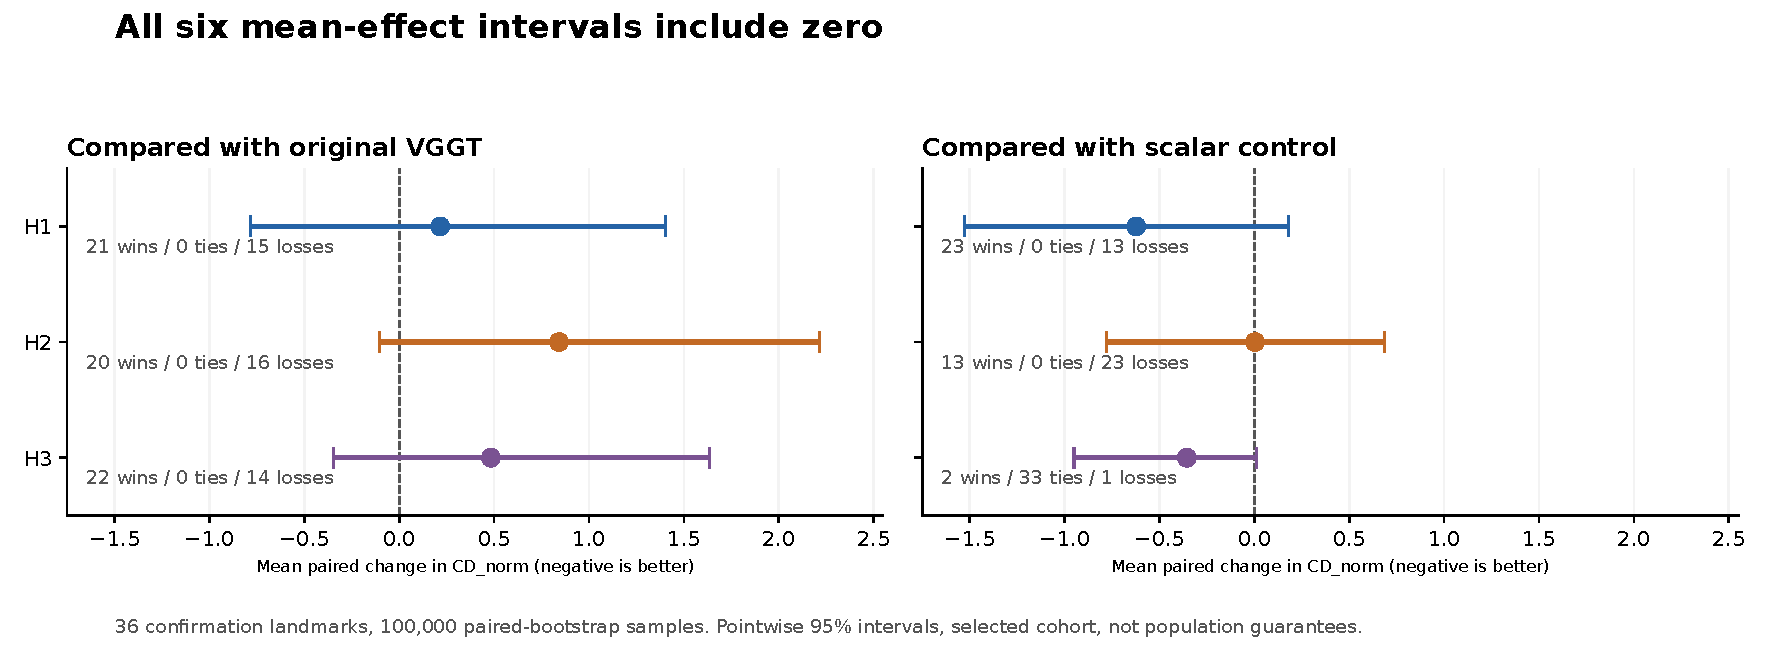
\includegraphics[width=\textwidth]{figures/extended_paired_effects.pdf}
\caption{Mean paired differences and pointwise 95\% landmark-bootstrap intervals against both references. The zero line denotes no mean change. H1 has the most favorable mean against the scalar, while the original model retains the lowest cohort mean error.}
\Description{Two panels show H1, H2, and H3 mean differences and bootstrap intervals against original VGGT and scalar steering. Every interval crosses zero.}
\label{fig:bootstrap}
\end{figure*}

H1's scalar-relative advantage survives every single-landmark omission, but the original-model comparison is sensitive to Pal\'acio Nereu Ramos. Removing that case changes H1's mean difference from $+0.2164$ to $-0.1884$. H2 and H3 remain worse than the original mean after every possible single omission. All 36 landmarks remain in the official scores. Omission is an influence diagnostic, not a revised result.

\paragraph{Exploratory feature search.}
We examine 28 primary continuous-feature associations using Spearman rank correlations and 18 categorical associations using rank-based permutation omnibus tests. Features include physical extent, variable strength coefficients, relative update magnitude, executed anchor, region, and building type. The 46 tests are pooled for Benjamini--Hochberg and Holm correction. None survives either global correction at 0.05. The smallest global BH $q$ is 0.09476. These analyses use the already-frozen confirmation outputs and do not fit a new selection rule.

The strongest categorical pattern is region for H1 relative to the scalar (raw $p=0.00206$, global $q=0.09476$). It passes correction within the smaller 18-test categorical family ($q=0.03708$), but not across the combined search. The corresponding original-model comparison has $p=0.41068$. North America has four scalar-relative wins from four landmarks and South Asia five from five. These small, overlapping geographic and architectural groups cannot identify a causal regional effect.

The strongest continuous hints are H3 relative-update magnitude versus its original-model difference ($\rho=+0.445$, raw $p=0.00672$, global $q=0.15456$), and H2 coefficient spread versus its scalar-relative difference ($\rho=-0.411$, raw $p=0.01412$, global $q=0.16238$). Positive associations indicate larger features accompany worse effects. Negative associations indicate better effects. Both retain their sign after each single-landmark omission, but neither establishes a usable predictor. For H3, 33 predictions duplicate the scalar, so the association mostly describes scalar behavior. For H2, 21 of 36 coefficient ratios tie at four. Average ranks handle those ties. The independently chosen base strengths also confound weighting with step magnitude.

Constant diagnostics were excluded. Every selected run accepted 24 layers, clipping counts were zero, and H1's mean relative update was essentially fixed at 0.02. View count is 50 for 35 landmarks and 26 for one, so it was not treated as an informative continuous predictor. Original error versus improvement shares an error term algebraically and is not evidence for a difficulty-based selector. Some H3--scalar bootstrap correlation samples contain only ties and have undefined correlation. Stored correlation intervals condition on defined samples. Additional log-ratio sensitivity checks provide no corrected discoveries.

\paragraph{Complementary successes.}
At least one hypothesis beats the original on 28 of 36 landmarks. All three beat it on 14 and none on eight. At least one beats both controls on 19 landmarks, while none of the landmarks is improved over both controls by all three methods. These counts identify complementary outcomes after observing ground truth. They do not measure the accuracy of an inference-time selector, and choosing the best observed method for each landmark would leak confirmation outcomes.

\subsection{Verified Reconstruction Examples}
\label{sec:qualitative-summary}
The exported confirmation examples are Herald Square for H1, Itmad-Ud-Daulah's Tomb for H2, and Marine Corps War Memorial for H3. Within each hypothesis, the case is selected post hoc as the largest percentage improvement over the original among landmarks that improve over both controls. They demonstrate possible gains, not typical performance. Table~\ref{tab:qualitative-cases} gives full-cloud numerical scores, and Appendix~\ref{app:qualitative} displays the reconstructions.

The nine re-exported conditions (original, scalar, and selected rule for each case) reproduce their recorded prediction hashes and metrics. Matched images, masks, and frozen settings are retained. Each displayed pair uses the same camera, point size, and framing, with real sampled geometry and no geometric smoothing. The H3 main view uses an explicitly shared scene crop because distant outliers otherwise dominate the framing. Its wide view is retained in the project. Crop selection does not change the full-cloud evaluation. These are whole-landmark comparisons, not separately scored anchor regions.

\begin{table*}[t]
\caption{Post-hoc qualitative cases. Scores are whole-landmark normalized Chamfer error, lower is better. Reductions are percentages for each selected landmark and do not replace the 36-landmark results.}
\label{tab:qualitative-cases}
\centering
\small
\begin{tabular}{lllrrrrr}
\toprule
Rule & Landmark & Anchor & Original & Scalar & Rule & \multicolumn{2}{c}{Reduction vs (\%)}\\
 & & & & & & Original & Scalar\\
\midrule
H1 & Herald Square & facade & 6.9134 & 6.5884 & 5.1401 & 25.65 & 21.98\\
H2 & Itmad-Ud-Daulah's Tomb & railing & 17.7941 & 23.6269 & 15.1476 & 14.87 & 35.89\\
H3 & Marine Corps War Memorial & statue & 31.6116 & 36.4341 & 28.0207 & 11.36 & 23.09\\
\bottomrule
\end{tabular}
\end{table*}

\subsection{Main Findings and Interpretation}
\label{sec:point3-findings}
The benefit of structured steering depends strongly on the landmark. H1 and H3 improve the calibrated scalar's mean error, but none of the tested rules beats original VGGT in mean across 36 confirmation landmarks. Improving an intervention does not necessarily improve on leaving the model unchanged.

\paragraph{H1 is the strongest candidate for improving the scalar rule.}
H1 reduces the scalar mean by 4.22\%, wins on 23 of 36 landmarks, and retains its mean advantage after every single-landmark omission. Its normalization targets a similar relative change in anchor activations across layers. The result is consistent with that motivation, without establishing the mechanism causing the gains. H1 remains 1.55\% worse than original VGGT in mean. Its scalar-relative bootstrap interval includes zero.

\paragraph{H2 shows that visible anchor area is not an established guide to useful steering.}
H2's mean is almost unchanged from the scalar (+0.03\%), with 13 scalar-relative wins. A possible explanation is that larger anchor masks indicate visibility without identifying where stronger updates help geometry. This interpretation is untested. H2 and the scalar also use different calibrated base strengths, preventing attribution of their difference to view weighting alone.

\paragraph{H3's benefit comes from three decisions.}
Only two statues and one column receive a different coefficient. The other 33 predictions duplicate the scalar. Two gains and one regression produce the entire 2.41\% mean reduction. Reducing strength helps particular cases, but this does not establish a successful anchor-dependent policy across all 23 confirmation labels.

\paragraph{Local successes coexist with costly failures.}
H1, H2, and H3 beat original VGGT on 21, 20, and 22 landmarks respectively, yet large regressions outweigh these wins in the mean. Pal\'acio Nereu Ramos is the largest regression for all three. Conversely, H1 improves all three facade-labeled landmarks against both controls, reducing their group mean by 16.80\% versus original VGGT. These are whole-landmark gains, not separately measured improvements within the anchor. Appendix~\ref{app:qualitative} shows selected successes for all three rules.

\paragraph{The evidence identifies leads, not a reliable selector.}
All six paired mean-effect intervals include zero, and none of 46 primary exploratory associations survives global correction. This matched evaluation identifies gains, failures, and their concentration. H1 offers the strongest observed improvement over the scalar. A rule predicting when to steer still requires independent evaluation. Choosing the winning method from confirmation outcomes would not demonstrate an inference-time selector.

\subsection{Possible Causes of Large Regressions}
\label{sec:regression-analysis}
The largest failures motivate a distinction between observed diagnostics and possible mechanisms. Table~\ref{tab:regression-diagnostics} reports saved scores and activation-update magnitudes for two informative cases. These observations do not identify a unique cause. The explanations below are hypotheses for targeted investigation, not established causal findings.

\paragraph{Attention-based acceptance does not guarantee better geometry.}
The inherited hook accepts an update when its monitored anchor-attention statistic rises. It does not check ground-truth geometry, depth consistency, or reconstruction error. All 24 intervened layers accepted their updates in the selected runs, including the largest failures. Therefore, the observed regressions coexist with success under the acceptance criterion. Increasing attention to an anchor can still alter representations in a way that harms the final geometric prediction. The common attention objective and acceptance rule are consequently plausible sources of failure across hypotheses.

\paragraph{The relative perturbation can be excessive for a particular scene.}
At Heian-jing\={u}, H1's mean applied update on anchor activations is 2.00\%, compared with 0.202\% under the scalar, approximately ten times larger. Error increases from 17.0083 to 24.6149. This makes excessive perturbation a plausible explanation for that H1 regression, but neither the magnitude ratio nor the error change proves causality. The percentages describe activation-norm ratios averaged across layers, not physical displacement or a cumulative percentage change through the network.

\paragraph{Magnitude alone does not explain all failures.}
At Pal\'acio Nereu Ramos, every selected intervention is worse than original VGGT. H2 produces the largest error, despite a mean relative update of only 0.194\%, compared with 2.00\% for H1 and 1.651\% for the scalar/H3. Thus a smaller recorded update does not guarantee a better outcome. Its direction, its allocation across views, and subsequent nonlinear model responses could matter. H3 uses the scalar fallback for this dome-labeled landmark, so its regression is inherited rather than a distinct category-selection failure.

\begin{table*}[t]
\caption{Observed failure-case diagnostics. Error is whole-landmark normalized Chamfer distance. Update percentages are the mean applied anchor-masked activation-norm ratios across the 24 layers, not displacement in 3D space. Original VGGT has no steering update. All displayed intervention runs accepted all 24 layers.}
\label{tab:regression-diagnostics}
\centering
\begin{tabular}{llrr}
\toprule
Landmark & Condition & Error & Mean relative update (\%)\\
\midrule
Pal\'acio Nereu Ramos & Original VGGT & 36.7702 & ---\\
Pal\'acio Nereu Ramos & Scalar / H3 & 52.7006 & 1.651\\
Pal\'acio Nereu Ramos & H1 & 51.1525 & 2.000\\
Pal\'acio Nereu Ramos & H2 & 56.4200 & 0.194\\
\midrule
Heian-jing\={u} & Original VGGT & 18.0656 & ---\\
Heian-jing\={u} & Scalar & 17.0083 & 0.202\\
Heian-jing\={u} & H1 & 24.6149 & 2.000\\
\bottomrule
\end{tabular}

\end{table*}

\paragraph{Anchor choice and mask quality remain possible contributors.}
The same anchor and masks are reused across hypotheses. A wrong or incomplete mask, inconsistent segmentation across views, or similarly labeled structures that are not corresponding physical points could make the shared objective unhelpful. Even a semantically correct anchor need not be the best guide for geometric reconstruction. The gradient update is not restricted to anchor tokens, so a problem with the anchor objective can affect the wider prediction. We have not established that the masks for these failure cases are incorrect. Complete semantic mask review remains outstanding.

\paragraph{Calibration does not provide a scene-level option to abstain.}
The rules were selected on 18 calibration landmarks from two positive candidate strengths per rule. They do not include a calibrated decision to choose original VGGT for a new scene. Although individual layer updates can be reverted when attention fails to rise, that mechanism did not reject the updates in these cases. A setting preferred on the calibration set can therefore transfer poorly to a confirmation landmark. H3's fallback can also preserve a harmful scalar choice.

\paragraph{Geometry, outliers, and alignment need separate inspection.}
The evaluator measures mean nearest-neighbor distances after similarity alignment and ICP refinement. Distorted surfaces, distant points, or a changed alignment may increase that mean substantially. ICP is a local procedure whose convergence depends on initial alignment~\cite{open3d_icp}. This motivates inspecting the failure cases' clouds and alignment outputs. It does not establish an evaluation artifact or invalidate their reported scores. Matched-input and numerical checks passed, but those checks do not identify the geometric reason for a regression.

\paragraph{Targeted diagnostics.}
The most informative next checks are mask overlays and paired reconstructions for Pal\'acio Nereu Ramos and Heian-jing\={u}, pointwise error distributions and the separate accuracy/completeness terms, and alignment quality before and after ICP. A small strength sweep including zero intervention, with a matched-strength scalar control for H2, could then distinguish magnitude and view-weighting effects. These are proposed diagnostics. No additional runs or confirmation-based retuning enter the reported results.

\subsection{Findings Established by the Saved Runs}
\label{sec:saved-findings}
The absence of an established population-level improvement does not make every result inconclusive. The following descriptive findings use the same frozen outputs, retain all 36 confirmation landmarks, and require no additional model runs. They distinguish observed behavior from causal explanations and hypothetical selection performance.

\paragraph{Attention-based acceptance did not screen out harmful reconstructions.}
All 24 layers accepted their updates on all 36 selected runs for each hypothesis. Nevertheless, whole-landmark error exceeded original VGGT on 15 H1, 16 H2, and 14 H3 landmarks. Thus a rise in the monitored attention statistic is demonstrably insufficient to guarantee improved geometry in this cohort. This is an observed limitation of the acceptance criterion, not proof that attention itself caused the errors. The three method-specific counts are not independent samples, especially where H3 duplicates scalar predictions.

\paragraph{A few regressions account for most of the error increases.}
For each method, we separate paired changes from original into gross gains and gross harms. H1's improvements contribute a mean error reduction of 0.7627, while its regressions contribute an increase of 0.9791, leaving the reported net increase of 0.2164. The three largest regressions account for 74.24\% of H1's gross harm, 74.32\% of H2's, and 86.44\% of H3's. These percentages divide the sum of the three largest positive differences by the sum of all positive differences. They are not percentages of total reconstruction error. The worst cases are identified post hoc and remain in every headline mean.

\paragraph{The tested predictions contain gains that our selectors do not recover.}
For diagnosis only, define an observed-candidate oracle that chooses the smallest recorded error for each landmark after seeing ground truth. Selecting among scalar, H1, H2, and H3 gives mean error 13.3201, 4.34\% below original VGGT. Adding original VGGT as an option gives 12.8996, a 7.36\% reduction. At least one intervention beats original on 28 landmarks. Original is best on the other eight. These numbers quantify available gains within the measured candidate set. They are hindsight references, not achieved selector performance, and are not a full strength-sweep oracle.

An ideal choice restricted to H1 or original gives mean error 13.1615, 5.48\% below original. Its gain is 74.44\% of the full observed-candidate oracle gain. This motivates studying when to abstain from H1, as well as which structured method to use. It does not demonstrate that a practical abstention rule can recover that gain. Table~\ref{tab:saved-oracle} separates implemented methods from these hypothetical choices.

\begin{center}
\begin{minipage}{\columnwidth}
\captionof{table}{Confirmation means and hindsight diagnostics. Lower is better. Oracle choices use ground-truth errors and cannot be reported as achieved inference-time policies.}
\label{tab:saved-oracle}
\centering
\small
\begin{tabular}{lr}
\toprule
Method or diagnostic & Mean error\\
\midrule
Original VGGT & 13.9243\\
H1 everywhere & 14.1406\\
\midrule
Oracle, four interventions & 13.3201\\
Oracle, H1 or original & 13.1615\\
Oracle, all five options & 12.8996\\
\bottomrule
\end{tabular}

\end{minipage}
\end{center}

\paragraph{An available matched-strength H2 comparison exposes counterexamples.}
The saved H3 runs provide scalar $\eta=100$ predictions for three confirmation landmarks, allowing comparison with H2 at base $\eta=100$ under the matched study inputs. H2 is worse on Mansudae Grand Monument (5.7559 versus 5.1155), Marine Corps War Memorial (30.0137 versus 28.0207), and Palacio Legislativo, Uruguay (23.0705 versus 16.9522). Their mean rises from 16.6961 to 19.6134, or 17.47\%. These cases show that view weighting can hurt even when base strength is matched. They are two statues and one column selected by H3's lookup, so they do not estimate the full-cohort effect of view weighting. The separate 18-landmark calibration comparison has an 8.15\% lower H2 mean, but is in-sample and is not pooled with confirmation.

\subsection{Exploratory Selection with Complete Cohort Coverage}
\label{sec:complete-selection}
To assess whether group-specific preferences justify selection, we also examine three simple rules over the existing anchor, building-type, and region categories. Each chooses the lowest mean calibration error among the frozen scalar/H1/H2/H3 candidates when a category has at least two calibration landmarks. Otherwise it uses the best global calibration candidate, H3. Exact-anchor selection has direct support on 17 confirmation landmarks and falls back on 19. Building-type selection has support on 24 and falls back on 12. Region has support on all 36. No landmark is omitted from their aggregate scores.

An additional fixed rule chooses the best mean-error method among each scene's three nearest calibration landmarks in the saved image-derived appearance distance. It uses neither the two-dimensional visualization coordinates nor the composite distance containing physical extent, and performs no neighbor-count search. Every confirmation landmark receives a choice, including rare anchors. The descriptor extraction belongs to the prior dataset-selection procedure. Equivalence to the reconstruction's sampled views and compute budget has not been established.

The confirmation means are 14.2396 for anchor selection, 14.1574 for building-type selection, 14.5274 for region selection, and 14.4054 for appearance-neighbor selection. All improve the scalar mean of 14.7630. None improves H1's 14.1406 or original VGGT's 13.9243. Appearance selection chooses H1 on 28 landmarks, H2 on one, and H3 on seven. Its eight departures from H1 yield one improvement and seven regressions. Providing a choice for every scene therefore does not establish useful selection.

These audits were initiated after inspecting confirmation outcomes. Although fitting uses calibration errors only, this remains retrospective exploration rather than a new blinded evaluation. Original-VGGT calibration errors are absent from the score tables used by these audits, so the rules cannot learn when to choose no intervention. Their candidates were themselves calibrated on the same 18 landmarks. No new significance claim is made, and the earlier correction over 46 associations does not cover a further search over selection rules. Complete per-landmark decisions, coverage counts, and source hashes accompany the report under \nolinkurl{extended_evidence/selection/} and \nolinkurl{extended_evidence/saved_findings/}.


\subsection{Limitations and Remaining Validation}
\label{sec:structured-limitations}
\paragraph{Scope and uncertainty.}
This is one frozen 18/36 allocation and one image-sampling seed, with only two candidates per structured rule. We report paired effects and conditional bootstrap intervals. None of the six pointwise intervals excludes zero. The analyses do not establish population-level superiority. The coverage-driven subset deliberately overrepresents rare anchors and does not provide probability-sampling weights for the benchmark. Anchor subgroups are especially small. 17 of 23 contain a single confirmation landmark. Their differences can reflect landmark identity, scene difficulty, or mask quality as well as the anchor label. The post-hoc subgroup comparisons do not establish causal architectural effects or corrected statistical significance. Multi-seed repeats and broader evaluation remain outstanding.

\paragraph{What the controls establish.}
The combined validator establishes numerical comparability, including exact agreement of repeated controls. It does not establish correct semantic segmentation or a successful intervention on every architecture type. Three selected confirmation reconstructions have been exported and verified (Appendix~\ref{app:qualitative}). Complete mask-overlay review is still pending. A rise in anchor attention is not itself proof of improved geometry, as the mean-error comparisons illustrate.

\paragraph{Oracle and final-evaluation limits.}
The study compares structured rules with no intervention and a calibration-selected scalar. It does not contain a matched five-value oracle sweep on all 36 confirmation landmarks. Consequently, these results do not quantify how much of the full oracle gap the structured rules close. The separate 79-landmark evaluation pool was not run by this study, and the promised full-396 evaluation is not complete. Before a team-wide final test, the split must be reconciled with earlier team experiments. 15 of those 79 IDs appear in their development/test lists. The pool is unused by this contribution but cannot be described as untouched across the whole team.

\subsection{Reproducibility}
The report includes per-landmark results, frozen selections, calibration scores, diagnostics, and subset-audit evidence. The script \nolinkurl{reproduce_results.py} checks sample identities, calibration-only choices, counts, shared controls, and aggregate tables without a GPU. Its optional \texttt{--plots} flag regenerates the original results figures. The companion script \nolinkurl{anchor_analysis/analyze_by_anchor.py} verifies the confirmation labels against the frozen plan and regenerates all anchor tables, win/tie/loss counts, individual-case summaries, and omission-sensitivity ranges. Its optional \texttt{--plots} flag regenerates the anchor figures. Both scripts use the saved numerical evidence without rerunning inference. The additional CPU analyses, their settings, and checked source snapshot are supplied in the companion \nolinkurl{Point3_Extended_Analysis.zip}. Selected result tables are also included under \nolinkurl{extended_evidence/} in this project. The reconstruction exports reproduce all nine original condition hashes and metrics across the three illustrated landmarks. The recorded experiment source hash begins \texttt{145b9848b597}. The executed notebook bundle checksum begins \texttt{04096da1573e}. These identify different artifacts and are not interchangeable.
